% ********** Chapter 1 **********
\chapter{Java und PHP}
\label{sec:chap1}

In diesem Kapitel soll eine JSR-223 Implementierung f"ur PHP entworfen und erarbeitet werden. Hierzu wird zun"achst
die Aufgabe analysiert und die Anforderungen die diese stellt er"ortert. Diese Anforderungen werden dann genutzt
um das Vorgehen bei der Implementierung zu planen, und um eine Architektur zu entwerfen die diese Anforderungen 
m"oglichst komplett erf"ullt. Schliesslich werden die gewonnenen Erkenntnisse genutzt um die erarbeitete Vorgehensweise
in die Tat zu setzen und eine Bibliothek zu erstellen, die es dem Anwender erlaubt PHP-Skripte in Java auszuf"uhren,
Daten an diese Skripte zu senden, aus Java heraus PHP-Funktionen aufzurufen, und aus diesen Skripten heraus 
Java-Funktionalit"at zu nutzen.

% ********** Chapter 1 **********
\section{Analyse}
\label{sec:chap1:ana}

In diesem Abschnitt wird erl"autert wie der erste Teil der Aufgabenstellung analysiert wurde, welche Use-Cases dabei gefunden 
wurden, und wie aus diesen Use-Cases Arbeitspakete abgeleitet wurden. Dieser erste Teil umfasste haupts"achlich das Ausf"uhren 
von PHP-Sourcecode innerhalb einer Java-Anwendung. 
Die Anforderung war m"oglichst grosse Teile des XP-Frameworks innerhalb von Java auszuf"uhren.
Vom vollen Umfang des XP-Frameworks ausgenommen waren lediglich die Komponenten welche eine Kommunikation
nach aussen erlaubten, so zum Beispiel die Datenbankkonnektivit"at, da diese Funktionen sp"ater vom Application Server
bereitgestellt werden sollten. Idealerweise sollte die verwendete PHP Version leicht austauschbar sein. Eine weitere
Anforderung war die Interaktion von Java nach PHP und umgekehrt m"oglichst einfach zu gestalten, Java-Objekte sollen
in PHP erzeug- und zugreifbar sein.

\subsection{Use-Cases}
\label{sec:chap1:ana:uc}

Use-Cases (auch Anwendungsf"alle) definieren die Interaktion zwischen Akteuren und dem zu entwerfenden Softwaresystem.
Das Erstellen der Use-Cases soll nicht nur zu einem Besseren Verst"andnis der zu implementierenden Abl"aufe, sondern
zu einem besseren Verst"andnis der gesammten Aufgabe f"uhren. Zun"achst mussten allerdings die m"oglichen Akteure ermittelt
werden, und es ergab sich dass lediglich zwei unterschiedliche Akteure existieren: der Java-Anwender, der eine Java-Applikation
benutzt beziehungsweise entwickelt und den PHP-Anwender, dessen PHP-Skript aus Java heraus ausgef"uhrt wird. Auf oberster Ebene
wollen diese beiden Akteure Daten austauschen, beziehungsweise auf Eingaben des einen reagieren um Ergebnisse zur"uckzuliefern,
bei genauerer Betrachtung lie\ss en sich im Wesentlichen vier Use-Cases aus der Aufgabe ableiten:

\begin{figure}[h]
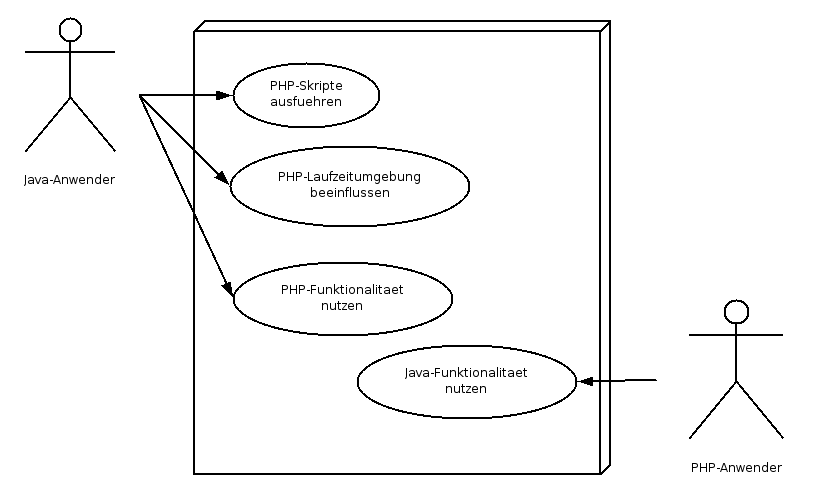
\includegraphics[width=\textwidth]{chap1/img/usecases.png}
\caption{Use-Cases}
\label{fig:usecases}
\end{figure}

\begin{description}
    \item[UC.01 - Ausf"uhren von PHP-Skripten] Ein Java-Anwender m"ochte ein oder mehrere PHP-Skripte aus einer
        Java-Applikation heraus ausf"uhren. Hierbei soll es m"oglich sein das Skript zur Laufzeit der Java-Applikation
        zu ver"andern und erneut auszuf"uhren. Weiterhin sollen Daten sowohl aus Java an das PHP-Skript "ubergeben, als
        auch Ergebnisse des Skriptes an Java zur"uck"ubergeben werden.
    \item[UC.02 - Beeinflussen der PHP Laufzeitumgebung] Es soll dem Java-Anwender m"oglich sein Einfluss auf die PHP-Laufzeitumgebung
        zu nehmen. Dies geschieht bei PHP typischerweise durch das Setzen von Initialisierungsparametern, entweder Systemweit
        in der Datei "'php.ini"', beim Starten des PHP-Interpreters, oder zur Laufzeit des PHP-Skriptes.
    \item[UC.03 - Zugriff auf Java aus PHP] Dem Entwickler eines PHP-Skriptes soll Zugriff auf m"oglichst den kompletten 
        Funktionalit"atsumfang der Java-Umgebung gew"ahrt werden. Das umfasst vor allem das Instanziieren von Java-Objekten und
        den Zugriff auf deren Methoden und Attribute, aber auch weitere Sprachfunktionen wie beispielsweise das Werfen und 
        Fangen von Exceptions. Zus"atzlich soll der Zugriff auf Java f"ur den PHP-Anwender m"oglichst intuitiv ablaufen, im
        Idealfall sollen sich Java-Objekte in PHP genauso behandeln lassen wie native PHP-Objekte.
    \item[UC.04 - Zugriff auf PHP aus Java] Es soll einem Java-Entwickler erm"oglicht werden auf einfach Art und Weise auf
        innerhalb eines PHP-Skriptes vorhandene Funktionen, Klassen und deren Methoden zuzugreiffen. Auch hier soll
        dieser Zugriff m"oglichst intuitiv erfolgen, PHP-Objekte sollen sich wie Java-Objekte benutzen lassen. 
\end{description}

\subsection{Anforderungen}
\label{sec:chap1:ana:ap}

Nachdem die Use-Cases bekannt waren musste festgelegt werden welche Einzelanforderungen sie jeweils an das System stellen.
Im Gegensatz zu den Use-Cases, die die Sicht des Anwenders auf das System darstellen, sollte dieser Schritt der Analyse
die n"otigen Funktionen ergeben, die das System bereitstellen muss, um die Anforderungen des Anwenders zu erf"ullen.
Weiterhin soll f"ur jede dieser Anforderungen beschrieben werden, wie ein Test aussehen k"onnte der ermittelt, ob die 
Anforderung erf"ullt ist.

\begin{enumerate}
\item Die PHP-ScriptEngine muss f"ur den Anwender verf"ugbar sein. Die aktuelle Java-Umgebung muss so konfiguriert sein,
    dass die PHP-ScriptEngine vom ScriptEngineManager "uber die in \ref{sec:javanscripts:jsr} beschriebenen Auffindungsmechanismen
    gefunden und instaziiert werden kann. Diese Anforderung ist eigentlich Grundlage des kompletten Systems, streng genommen wird sie
    aber nur von \emph{UC.01} gestellt.
    \textbf{Test}: Durch einfache Ausgabe auf der Konsole soll schnell ermittelbar sein, welche ScriptEngines geladen und einsatzbereit sind.

\item "Ubersetzen von PHP-Quelltext. Dem System "ubergebener PHP-Quelltext soll Gem"a\ss des in \texttt{javax.script} vorhandenen 
    Interfaces \texttt{Compilable} in eine ausf"uhrbare Form "ubersetzt werden. Das Ergebnis eines solchen "Ubersetzungsvorganges
    soll mehrfach ausgef"uhrt werden k"onnen.Beim "Ubersetzen auftretende syntaktische oder semantische Fehler sollen dem Anwender 
    als Java-Exception zur"uckgegeben werden.
    Auche diese Anforderung ist eine Vorraussetzung fast aller weiterer Anforderungen, weswegen sie ebenfalls \emph{UC.01} zugeordnet wird.
    \textbf{Test}: die "Ubergabe fehlerhaften PHP-Quelltextes soll zu einer Java-Exception f"uhren.

\item Ausf"uhren beliebiger PHP-Skripte. Es soll dem Anwender m"oglich sein, beliebige PHP-Skripte auszuf"uhren. Diese Skripte sollen
    in vielfacher Form an das System "ubergeben werden k"onnen, auch ohne dass der Anwender selbst Java-Quelltext schreiben muss.
    Zur Laufzeit des PHP-Skriptes auftretende Fehler sollen ebenfalls als Java-Exception an den Anwender weitergereicht werden.
    Aufbauend auf die beiden vorherigen Anforderungen realisiert diese Anforderung die in \emph{UC.01} geforderte Funktion.
    \textbf{Test}: Es soll auf der Kommandozeile der Name einer Datei "ubergeben werden, deren Inhalt als PHP-Skript ausgef"uhrt wird.

\item Datenaustausch. Zwischen den beiden Programmiersprachen soll der Austausch beliebiger Daten m"oglich sein. Simple (skalare)
    Datentypen sollen in ihre jeweilige Entsprechung in der anderen Sprache umgewandelt werden, komplexe Datentypen sollen in der anderen 
    Sprache als Referenz verf"ugbar sein. Auch die Daten"ubergabe mittels des vom JSR 223 definierten ScriptContext soll m"oglich sein.
    Sowohl \emph{UC.03} als auch \emph{UC.04} stellen diese Anforderung. 
    \textbf{Test}: Ein Mittels des Kontextes "ubergenes Java-Objekt soll in PHP ver"andert werden, und diese "Anderungen sollen in
    Java ausgelesen werden.

\item Erzeugen von Java-Objekten. Innerhalb eines ausgef"uhrten PHP-Skriptes soll es m"oglich sein Java-Objekte zu erzeugen und auf
    deren Methoden und Attribute zuzugreiffen. Dieser Zugriff soll f"ur den PHP-Anwnder m"oglichst einfach und intuitiv m"oglich sein.
    Diese Anforderung ist ein wesentlicher Teil von \emph{UC.03}.
    \textbf{Test}: Es soll ein Skript aufgerufen werden, welches ein Java-Objekt erzeugt, eine Methode dieses Objektes aufruft und
    deren Ergebnis an die Java-Applikation zur"uckgibt.

\item Java-Exceptions. Neben dem Zugriff auf Java-Objekte soll es dem PHP-Anwender auch m"oglich sein aus einem
    PHP-Skript heraus beliebige Java-Exceptions zu werfen. Diese Exceptions sollen entweder wie andere Java-Objekte auch vor dem Werfen,
    oder beim Werfen selbst aus einem "ubergebenen Klassennamen erzeugt werden. Dem PHP-Anwender soll ebenfalls erm"oglicht werden
    zu "uberpr"ufen ob Java-Exceptions aufgetreten sind, und aufgetretene Java-Exceptions abzuarbeiten.
    Diese Anforderung wird explizit vom \emph{UC.03} gestellt.
    \textbf{Test}: Es soll ein PHP-Skript ausgef"uhrt werden das eine Java-Exception provoziert, und auf diese Exception reagiert.

\item Weitere Java-Funktionalit"at. Implizit fordert \emph{UC.03} ebenfalls dass das System dem PHP-Anwender erlaubt grundlegende
    Funktionalit"at der Java-Umgebung zu nutzen, so soll er "uberpru"ufen k"onnen ob ein Java-Objekt identisch mit einem anderen ist
    (\texttt{equals()}), ob es Instanz einer bestimmten Klasse ist (\texttt{instanceof}), oder ob es sicher auf eine andere Klasse castbar ist.
    \textbf{Test}: Innerhalb eines PHP-Skriptes sollen auf einem Java-Objekt jeweils die oben genannten Tests durchgef"uhrt werden.

\item Aufrufen von Methoden in "ubersetzten Skripten. Das zu entwickelnde Softwaresystem soll das Aufrufen sowohl von globalen Funktionen,
    als auch von Objektmethoden in "ubersetzten PHP-Skripten aus Java heraus erlauben, hierzu soll das Interface \texttt{javax.script.Invocable} 
    implementiert werden. Die "Ubergebenen Funktions- und Methodenargumente sollen wie schon beim Datenaustausch in ihre PHP-Entsprechungen
    umgewandelt werden. Diese Anforderung stellt einen wesentlichen Teil des \emph{UC.04} dar.
    \textbf{Test}: Es soll aus einer Java-Applikation heraus eine PHP-Funktion aufgerufen werden die ein PHP-Objekt zur"uckgibt, welches
    ein Java-Interface implementiert. Auf diesem Objekt soll dann eine Interface-Methode aufgerufen werden.

\item Setzen von php.ini Parametern. Dem Anwender soll die M"oglichkeit geboten werden gezielt php.ini Werte zu setzen oder zu verwenden,
    um das Laufzeitverhalten von PHP wie gewohnt zu beeinflussen. Diese Werte sollen aus den Java-Systemproperties ausgelesen werden,
    da diese sowohl zur Laufzeit der Java-Applikation programmatisch als auch vor dem Start der Java-VM beispielsweise "uber die Kommandozeile
    gesetzt werden k"onnen. Die php.ini ist der gew"ohnliche Weg das Laufzeitverhalten des PHP-Interpreters zu ver"andern, somit werden
    die Anforderungen die der  \emph{UC.02} stellt komplett erf"ullt.
    \textbf{Test}: Es soll der Wert php.ini-Wert \texttt{include\_path} "uber die Kommandozeile gesetzt und in einem
    PHP-Skript ausgelesen werden. 

\end{enumerate}

Nat"urlich decken die oben aufgelisteten Anforderungen nur die grundlegende Funktionalit"at des Systems ab, im Lauf der Implementierung werden
noch weitere notwendige oder auch nur n"utzliche Funktionen gefunden und realisiert werden.
% ********** End of chapter **********

\clearpage
% ********** Chapter 1 **********
\section{Design}
\label{sec:chap1:design}

Eine JSR 223-Implementierung f"ur PHP besteht gezwungenermassen aus zwei Teilen: Zum einen einem Java-Teil, welcher im Wesentlichen
die ScriptEngineFactory enth"alt. Dieser ist komplett in Java ohne die Verwendung von nativen (JNI-) Aufrufen implementiert und
deckt s"amtliche Funktionalit"at des Auffindungsmechanismus ab. Zum anderen einem nativen Teil, welcher aus 
einem C- oder C++ - Programm, das die n"otigen Aufrufe an PHP vornimmt, besteht.
Die eigentliche ScriptEngine verbindet diese beiden Teile, indem sie aus Java heraus dieses in nativen Code "ubersetzte 
Programm mittels JNI anspricht.
Um allerdings JSR 223 "uberhaupt nutzen zu k"onnen, m"ussen alle Klassen aus dem Package \texttt{javax.script}
im Java-Classpath liegen, damit dem Anwender der Zugriff auf die ScriptEngine "uber den ScriptEngineManager m"oglich ist.
Hierzu kann entweder eine Java-Runtime der Version 6 oder aber eine eigene Implementierung dieser Klassen genutzt werden. 
Die im folgenden beschriebene JSR 223 Implementierung tr"agt den Namen "'Turpitude"'.

\subsection{Java-Teil}
\label{sec:chap1:design:java}

Eine JSR 223-Implementierung muss sich um f"ur den ScriptEngineManager auffindbar zu sein gem"a\ss\ der 
\emph{Jar File Specification} \cite{JARSPEC} als sogenannter \emph{Service Provider}\footnote{
Ein \emph{Service Provider} ist eine spezifische Implementierung eines Interfaces oder einer abstrakten Klasse
} registrieren. Hierzu muss sich im Verzeichnis \texttt{META-INF/services} des Archivs eine Datei
mit dem Namen der Service-Klasse (in diesem Fall \texttt{ScriptEngineFactory}) befinden, in welcher verf"ugbare 
ScriptEngineFactories zeilenweise aufgelistet werden.

Das Package \texttt{net.xp\_framework.turpitude} enth"alt alle Klassen der Implementierung. 
Die ScriptEngineFactory-Implementierung hei\ss t \texttt{PHPScriptEngineFactory} und implementiert direkt das Interface 
\texttt{ScriptEngineFactory} aus \texttt{javax.script}. Im Gegensatz dazu implementiert die Klasse \texttt{PHPScriptEngine} nicht
direkt das Interface \texttt{ScriptEngine}, sondern erbt von der abstrakten Klasse \texttt{AbstractScriptEngine}. Diese bringt f"ur
viele Varianten der \texttt{eval()}-Methode schon eine Realisierung, sowie mit der Klasse \texttt{SimpleScriptContext} schon einen 
\texttt{ScriptContext} mit. Um den "ubergebenen Skriptcode tats"achlich auszuf"uhren, muss dieser an den mittels der Java-Methode
\texttt{System.loadLibary()} geladenen nativen Teil der Implementierung weitergegeben werden. Die Kommunikation mit diesem
nativen Teil findet mittels JNI-Methoden statt.
Weiterhin implementiert die PHPScriptEngine die beiden in \texttt{javax.script} enthaltenen Interfaces \texttt{Compilable} und
\texttt{Invocable}, deren Funktionalit"at zur Erff"ullung einiger der Use-Cases ben"otigt wird. F"ur die Methoden aus
Compilable wird noch eine weitere Klasse - \texttt{PHPCompiledScript} - erstellt, welche direkt von der abstrakten
Klasse \texttt{javax.script.CompiledScript} erbt.
Der Standard schreibt zwar vor, dass die ScriptEngine das Interface Invocable implementiert, allerdings ergibt das aus Sicht
des Autors nur wenig Sinn. Es bleibt unklar auf welchem der "ubersetzten Skripte Methoden und Funktionen aufgerufen werden sollen.
Aus diesem Grund wird neben der \texttt{PHPScriptEngine} auch das \texttt{PHPCompiledScript} dieses Interface implementieren
und Aufrufe der Interfacemethoden bei der \texttt{PHPScriptEngine} werden an das zuletzt "ubersetzte Script weitergeleitet.

Die Kommunikation zwischen Java und PHP findet "uber zwei unterschiedliche Kan"ale statt:
Bei der R"uckgabe von Daten aus einem PHP-Skript werden diese einfach kopiert, wobei primitive Datentypen (bool, long, double und string)
einfach in ihre Java-"Aquivalente (java.lang.Boolean, java.lang.Long, java.lang.Double und java.lang.String) umgesetzt werden.
Da alle Arrays in PHP assoziativer Natur sind, werden sie als untypisierte \texttt{java.util.HashMap} zur"uckgegeben, was bedeutet dass sowohl 
Schl"ussel als auch Wert vom Typ \texttt{java.lang.Object} sind. Einzig f"ur PHP-Objekte wird eine gesonderte Java-Klasse ben"otigt: \texttt{PHPObject}.
Sie enth"alt neben dem Klassennamen auch alle Eigenschaften eines PHP-Objektes. 
Diese werden in einer HashMap gespeichert, mit dem Namen der Eigenschaft als Schl"ussel.
\begin{floatingtable}{
\begin{tabular}{|l|l|}
\hline
Java-Typ & PHP-Typ\\
\hline\hline
jlong & long\\
jint & long\\
jshort & long\\
jchar & long\\
jbyte & long\\
jboolean & bool\\
jfloat & double\\
jdouble & double\\
jstring & string\\
jobject & TurpitudeJavaObject\\
jclass & TurpitudeJavaClass\\
type[] & TurpitudeJavaArray\\
\hline
\end{tabular}}
\caption{Typkonversion Java nach PHP}
\end{floatingtable}
Leider l"asst die JSR 223-Spezifikation sehr viele Fragen unbeantwortet, so wird beispielsweise zur Typkonversion nur lapidar auf 
Implementierungsdetails verwiesen. Da der Datenaustausch zwischen PHP und Java allerdings einen nicht unwesentlichen Bestandteil
einer JSR223-Implemenation darstellt, muss gezwungenerma\ss en eine Konvention gefunden werden. Diese wird in den Tabellen 4.1 und 4.2
erl"autert, sowohl von Java nach PHP als auch umgekehrt. Weiterhin wird bei der Typkonversion von PHP nach Java zwischen 
Methodenaufrufen und Werter"uckgaben unterschieden. Bei Methodenaufrufen wird versucht, in simple Datentypen wie \texttt{int} und \texttt{double}
umzuwandeln. Weil der aber Standard oft verlangt dass Objekte zur"uckgegeben werden, wird bei der R"uckgabe von Werten in den entsprechenden
Objektyp wie zum Beispiel \texttt{java.lang.Boolean} konvertiert. Einige Java-Klassen und PHP-Objekte werden speziell konvertiert was
in den Tabellen gesondert aufgef"uhrt ist. Beispielsweise wird der
\texttt{java.lang.String} nicht zu einem \texttt{TurpitudeJavaObject}, sondern zu einem String in PHP. Die
Tabellen enthalten auch Verweise auf spezielle PHP-Klassen, die sp"ater im Kapitel \ref{sec:chap1:design:native} erl"autert werden.

\begin{table}
\begin{tabular}[tbh]{|l|l|l|}
\hline
PHP-Typ & Methodenaufruf & Werter"uckgabe\\
\hline\hline
long & jlong & java.lang.Long \\
double & jdouble & java.lang.Double \\
bool & jboolean  & java.lang.Boolean \\
array & java.util.HashTable & java.util.HashTable \\
object & PHPObject & PHPObject\\
constant & jstring & jstring\\
string & jstring & jstring \\
TurpitudeJavaClass & jclass & jstring\\
TurpitudeJavaObject & jobject & jobject\\
TurpitudeJavaArray & jarray & jarray\\
\hline
\end{tabular}
\caption{Typkonversion PHP nach Java, Methodenaufruf und Werter"uckgabe}
\end{table}

Die Eingabe von Daten aus Java heraus in ein PHP-Skript geschieht - gem"a\ss\ der JSR223-Spezifikation - mittels des Kontextes der
ScriptEngine. Hierzu wird dieser - zusammen mit einigen Umgebungsvariablen und -informationen - in eine globale Variable injiziert,
deren Name sich in der ScriptEngine setzen l"asst. Im Unterschied zu den oben beschriebenen R"uckgabewerten stellen die Kontext-Objekte
Referenzen dar, weshalb sich "Anderungen an diesen unmittelbar auf die entsprechenden Java-Objekte auswirken.

Die Abbildung \ref{fig:jsr223impl} zeigt die beteiligten Klassen und ihre Abh"anigkeiten untereinander,
zusammen mit einigen wichtigen Methoden und Attributen. 

\begin{figure}[h]
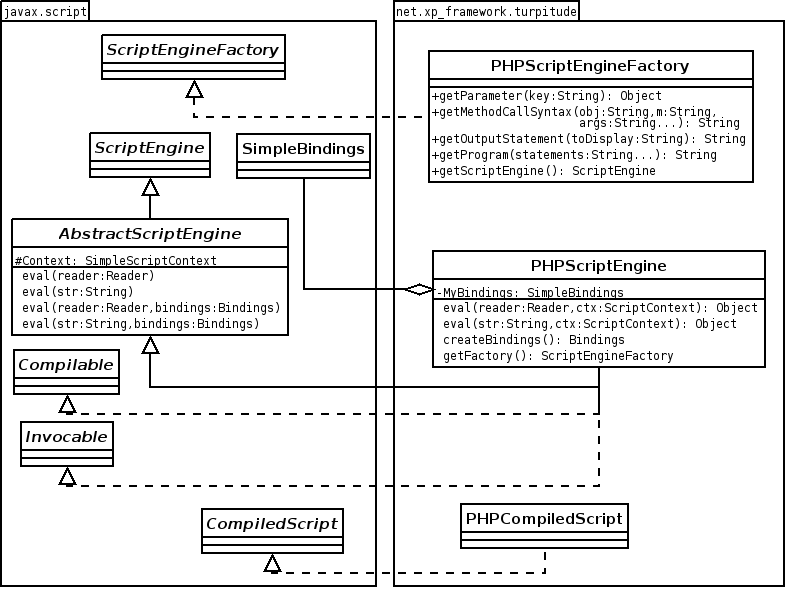
\includegraphics[width=\textwidth]{chap1/img/turpitude.png}
\caption{JSR 223 Implementierung - Architektur}
\label{fig:jsr223impl}
\end{figure}

Der JSR 223 spezifiziert lediglich eine einzige Exception (\texttt{ScriptException}) um alle m"oglichen Laufzeitfehler innerhalb einer 
Implementierung abzudecken. Um dem Anwender trotzdem eine M"oglichkeit einer differenzierten Fehlerauswertung zu geben, werden drei
zus"atzliche Exceptions eingef"uhrt: die \texttt{PHPScriptException}, die \texttt{PHPCompileException} und die \texttt{PHPEvalException} 
(siehe Abbildung \ref{fig:jsr223exceptions}). Die \texttt{PHPScriptException} dient zum Einen als Oberklasse, zum anderen kann der Anwender durch 
sie erkennen, ob das aufgetretene Problem implementationsspezifisch ist. Die beiden anderen neuen Exceptions werden genutzt um Fehler 
beim "Ubersetzen (\texttt{PHPCompileException}) oder beim Ausf"uhren (\texttt{PHPEvalException}) eines Skripts voneinander abzugrenzen.

\begin{figure}[h]
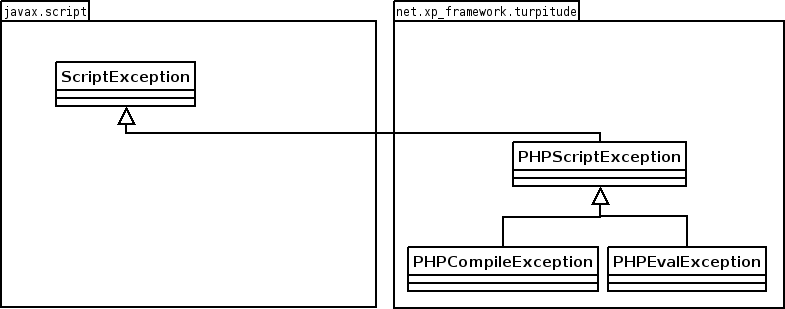
\includegraphics[width=\textwidth]{chap1/img/exceptions.png}
\caption{JSR 223 Implementierung - Exceptions}
\label{fig:jsr223exceptions}
\end{figure}

\subsection{Nativer/PHP-Teil}
\label{sec:chap1:design:native}

Der native Teil der Implementierung teilt sich wiederum auf in JNI-Methoden, f"ur welche die Headerdateien automatisch aus
der Java-Klasse der PHPScriptEngine generiert werden k"onnen, und in die Implementierung einer SAPI. Hierzu muss im
Wesentlichen ein sogenanntes \texttt{sapi\_module\_struct} angelegt und bef"ullt werden, welches neben einigen Strings
haupts"achlich Funktionspointer auf R"uckruffunktionen enth"alt, welche vom PHP-Interpreter aufgerufen werden. Da es
kaum m"oglich ist, dieses Konstrukt sinnvoll in eine objektorientierte Architektur einzuf"ugen, wird auf eine solche
vollst"andig verzichtet. Das \texttt{sapi\_module\_struct} und die dazugeh"origen Funktionen werden auf traditionelle,
prozedurale Art und Weise implementiert.

Die zu implementierenden SAPI-Funktionen ergeben sich aus den Anforderungen der Zend-API und sollen an dieser Stelle nur
sehr kurz erl"autert werden: die Funktionen \texttt{turpitude\_read\_cookies}, \texttt{turpitude\_flush}, \texttt{turpitude\_send\_headers},
\texttt{turpitude\_send\_header} und \texttt{turpitude\_log\_message} k"onnen leer, beziehungsweise auf triviale Art und Weise
implementiert werden, da sie f"ur den geplanten Einsatz der PHP-Umgebung keine Relevanz haben. Die Funktionen
\texttt{turpitude\_startup} und \texttt{turpitude\_register\_variables} leiten den Aufruf einfach an die entsprechenden
Zend-API Funktionen \texttt{php\_module\_startup} respektive \texttt{php\_import\_environment\_ variables} weiter, lediglich
die Funktion \texttt{turpitude\_error\_cb}, welche die R"uckruffunktion f"ur PHP-Laufzeitfehler darstellt, bedarf einer
komplizierteren Implementierung, da sie den PHP-Fehler als passende Java-Exception an den Anwender weitergeben soll.

Die JNI-Methoden ergeben sich aus dem Java-Quelltext, da sie Implementierungen von in Java als \texttt{native} deklarierten 
Methoden darstellen. Ihre Hauptaufgabe ist das Ausf"uhren von PHP-Quelltext beziehungsweise von PHP-Anweisungen.
Ausnahmen bilden lediglich die Methoden \texttt{startUp()} und \texttt{shutDown()} der PHPScriptEngine, welche
die Initialisierung beziehungsweise die kontrollierten Dekonstruktion der PHP-Laufzeitunmgebung und er Turpitude-spezifischen
Klassen "ubernehmen.

Um die Implementierung in PHP nutzen zu k"onnen muss auch hier eine Schnittstelle geschaffen werden. Leider schreibt
die Spezifikation keine API f"ur die Skriptseite vor, was zu einer Nichtaustauschbarkeit der Implementierung f"uhren kann.
Nichtsdestotrotz werden auf PHP-Seite folgende Klassen eingef"uhrt, welche im Wesentlichen JNI-Funktionen abbilden, und
in vielen F"allen auch die JNI-Syntax, zum Beispiel f"ur Java-Methoden, verwenden:

\textbf{TurpitudeEnvironment} - bietet neben der Methode \texttt{getScriptContext()}, die den JSR223 ScriptContext zur"uckgibt,
auch Schnittstellen an um grundlegende Java-Funktionalit"at aus PHP heraus anzusprechen:
\texttt{FindClass()} erzeugt die Repr"asentation einer Java-Klasse in PHP, \texttt{instanceOf()} "uberpr"uft, ob ein Java-Objekt 
Instanz einer bestimmten Java-Klasse ist. Weiterhin werden mit \texttt{throw()}, \texttt{throwNew()}, \texttt{exceptionOccurred()} und 
\texttt{exceptionClear()} Methoden angeboten, um Java-Exceptions zu werfen und zu fangen. TurpitudeEnvironment implementiert
das bekannte \emph{Singleton-Entwurfsmuster}, kann also nicht mehrfach existieren und wird zus"atzlich unter einem konfigurierbaren
Namen in das PHP-Superglobal\footnote{
Superglobals sind Variablen, auf die innerhalb eines PHP-Skriptes aus jedem Scope heraus zugegriffen werden kann. Superglobals k"onnen
nicht vom PHP-Anwender erzeugt werden, sondern werden von der PHP-Laufzeitunmgebung verwaltet.
} \texttt{\$\_SERVER} eingef"uhrt, in welchem laut dem PHP-Manual \cite{PHPMAN} SAPI-Informationen "uber die
Laufzeitumgebung gespeichert werden sollen.

\textbf{TurpitudeJavaClass} - PHP-Repr"asentation einer Java-Klasse, wird mittels der Methode \texttt{TurpitudeEnvironment::findClass()} erzeugt.
Bietet mit \texttt{findMethod()}, \texttt{findStaticMethod()} und \texttt{findConstructor()} M"oglichkeiten um gew"ohnliche Methoden, statische
Methoden und Konstruktoren der repr"asentierten Java-Klasse zu erzeugen. Weiterhin k"onnen mittels der Methode \texttt{create()} Instanzen
der Klasse erzeugt, und mittels der Methode \texttt{invokeStatic()} k"onnen statische Methoden der Klasse aufgerufen werden.
Enth"alt als Attribut den JNI-formatierten Klassennamen. 

\textbf{TurpitudeJavaMethod} - bildet eine Java-Methode in PHP ab. TurpitudeJavaMethod bietet selbst keine 
f"ur den Anwender aufrufbaren Methoden an und wird nur
als Parameter f"ur \texttt{TurpitudeJavaClass::create()} und beim Methodenaufruf auf Objekten und Klassen ben"otigt.
Als Attribute werden der Methodenname, deren Signatur sowie ein Indikator, ob die Methode statisch aufgerufen werden kann, vorgehalten.

\textbf{TurpitudeJavaObject} - repr"asentiert ein Java-Objekt, wird mittels der Methode \texttt{TurpitudeJavaClass::create()} erzeugt. Neben Methoden
die den sowohl lesenden als auch schreibenden Zugriff auf Attribute der Java-Klasse erlauben (\texttt{javaGet()} und \texttt{javaSet()}), k"onnen
auch direkt Methoden des gekapselten Java-Objektes mittels \texttt{javaInvoke()} aufgerufen werden. Falls m"oglich soll der Methodenaufruf aber
intuitiv nach folgendem Schema erlaubt werden:
\begin{lstlisting}[caption=angestrebte Syntax zum Aufruf von Java-Methoden in PHP]
$object->method($param1, $param2, ...);
\end{lstlisting}
R"uckgabewerte von Methodenaufrufen werden entweder auf skalare Typen in PHP oder wieder als TurpitudeJavaObject-Objekte abgebildet.
Eine Besonderheit bilden allerdings Java-Arrays: Diese k"onnten zwar als einfache Java-Objekte abgebildet werden, allerdings w"urde das 
nur den Zugriff auf Attribute erlauben, die allen Java-Arrays gemeinsam sind - wie beispielsweise \texttt{length}. Folglich muss eine weitere
Klasse eingef"uhrt werden, um dem Anwender auch den Zugriff auf die Elemente eines Java-Arrays zu erm"oglichen:

\textbf{TurpitudeJavaArray} - erlaubt den direkten Zugriff auf Elemente eines Java-Arrays in PHP. Allerdings k"onnen keine neuen Eintr"age
erzeugt werden, da Java-Arrays - anders als PHP-Arrays - nicht als HashMap, sondern als "'echte"' Arrays im Speicher abgebildet
sind, und eine Erweiterung dieses Bereiches nicht ohne Weiteres m"oglich ist. Der Zugriff auf diese Arrays soll nicht nur "uber 
Funktionen wie \texttt{get()} und \texttt{set()}, sondern auch "uber den Klammern-Operator [ ] m"oglich sein, um den Anwender einen
intuitiven Umgang zu bieten. Au\ss erdem soll das iterieren "uber Java-Arrays sowohl "uber die objektorientierte, in PHP5
enthaltene Schnittstelle \texttt{Iterator}, als auch "uber den normalen PHP-Operator \texttt{foreach} m"oglich sein. Das
\texttt{TurpitudeJavaArray} implementiert das PHP-Interface \texttt{IteratorAggregate}.

\textbf{TurpitudeJavaArrayIterator} - erlaubt das Iterieren "uber Java-Arrays in PHP. Der \texttt{TurpitudeJavaArrayIterator} implementiert
das PHP-Interface \texttt{Iterator} um das objektorientierte Iterieren "uber Java-Arrays zu erm"oglichen. Intern wird die aktuelle
Position im Array in einer einfachen Z"ahlvariable gespeichert. Wird diese gr"o\ss er oder gleich der L"ange des Java-Arrays wird der
Iterator ung"ultig und muss mittels \texttt{rewind()} zur"uckgesetzt werden. \texttt{next()} inkrementiert diesen Z"ahler um eins, die Methoden
\texttt{current()} und \texttt{key()} liefern das aktuelle Element beziehungsweise die aktuelle Position.

Der Zusammenhang zwischen Java-Arrays, den Turpitude-Klassen und PHP-Interfaces ist in der Abbilding \ref{fig:javaarrays} dargestellt.
Das von Java bereitgestellte Array wird in PHP in einem \texttt{TurpitudeJavaArray} gekapselt. Ein Aufruf der Methode
\texttt{getIterator()} erzeugt einen \texttt{TurpitudeJavaArrayIterator}, der intern eine Referenz auf das \texttt{TurpitudeJavaArray}
vorh"alt. 

\begin{figure}[h]
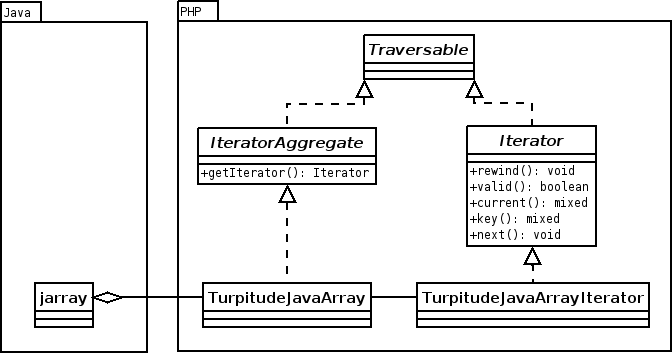
\includegraphics[width=\textwidth]{chap1/img/javaarrays.png}
\caption{Java-Arrays in PHP}
\label{fig:javaarrays}
\end{figure}

Ein typischer Ablauf eines PHP-Skriptes, welches auf Java-Objekte und Methoden zugreift, soll wie in Abbildung \ref{fig:phpseq} aufgezeigt 
aussehen:
Das \texttt{TurpitudeEnvironment} besteht "uber die komplette Laufzeit des Skriptes. Der Anwender erzeugt mittels der Methode \texttt{findClass()} 
des \texttt{TurpitudeEnvironment} eine \texttt{TurpitudeJavaClass} und ruft auf dieser die Methode \texttt{findConstructor()} auf, welche ihm 
eine Instanz der Klasse \texttt{TurpitudeJavaMethod} zur"uckgibt. Diese wiederum 
kann der Anwender der TurpitudeJavaClass beim Aufruf von \texttt{create()} "ubergeben, um schlussendlich eine Instanz der Klasse zu erzeugen.
Um nun auf dem Java-Objekt eine Methode aufzurufen, muss diese zun"achst wieder per \texttt{findMethod()} erzeugt werden, um dann der
Methode \texttt{javaInvoke()} zusammen mit den geforderten Parametern "ubergeben zu werden.

\begin{figure}[h]
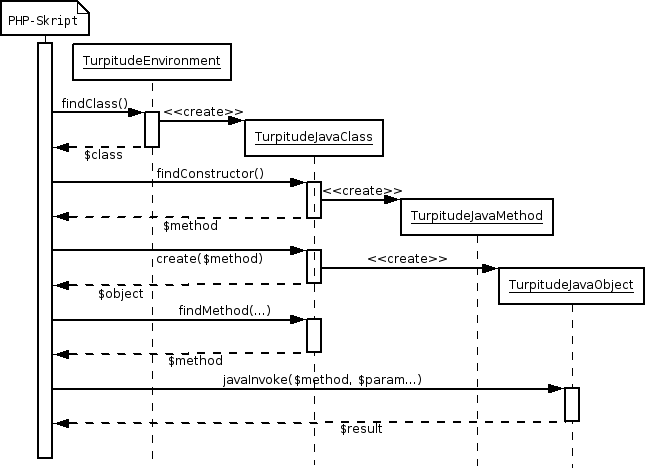
\includegraphics[width=\textwidth]{chap1/img/phpseq.png}
\caption{Ablauf eines PHP-Skriptes mit Zugriff auf Java-Objekte}
\label{fig:phpseq}
\end{figure}



% ********** End of chapter **********

\clearpage
% ********** Chapter 1 **********

\section{Implementation}
\label{sec:chap1:impl}

Um mit der Implementation beginnen zu k"onnen musste zun"achst ein als dynamisch ladbare Bibliothek verf"ugbares
PHP erzeugt werden. Hierzu wurde von \cite{PHPHP} ein PHP in der Version 5.2.0 im Quelltext heruntergeladen und 
"ubersetzt, nachdem es mittels des Kommandozeilenparameters "'--enable-embed=shared"' konfiguriert wurde. Die so
erzeugte \emph{libphp5.so} konnte, zusammen mit den vorhandenen Headerdateien, zur Entwicklung genutzt werden.

Nun musste noch daf"ur gesorgt werden, dass sich die vom JSR 223 verlangten Klassen aus \emph{javax.script} im
Classpath befinden. Nachdem allerdings die Klassen aus der Referenzimplementation aus den zum Teil in 
\ref{sec:chap1:prototype} beschriebenen Gr"unden nicht in Frage kamen, wurde von \cite{JAVAHP} ein
\emph{Java Development Toolkit (JDK)} der Version 6 heruntergeladen. Da dieses JDK nicht als System-VM genutzt
werden kann wurde ein Makefile erstellt, welches die zur "Ubersetzung und Ausf"uhrung n"otigen Kommandos
vereinfacht.

Nachdem diese Vorarbeiten geleistet waren konnte mit der eigentlichen Implementation begonnen werden.
Der erste Schritt war das Abbilden des ersten Use-Cases (verf"ugbare ScriptEngines auflisten), erstens um 
sicherzustellen dass die Entwicklungsumgebung den Anforderungen gerecht wird, und zweitens um einen ersten
Eindruck der JSR 223 API zu erhalten. Also wurde im Package \emph{samples} eine Klasse namens
\emph{EngineList} geschrieben, die einen ScriptEngineManager erzeugt, und mittels der Methode
\emph{getEngineFactories()} eine Liste aller verf"ugbaren ScriptEngines erstellt. Der Inhalt dieser
Liste wird dann mittels \emph{System.out.println()} ausgegeben. 
Nachdem dem Makefile ein Target namens "'list"' hinzugef"ugt wurde, ergab ein erstes Ausf"uhren dieser Klasse
zum einen keine Fehler, und zweitens dass dem JDK 6 mit \emph{Mozilla Rhino} bereits eine ScriptEngine beiliegt:
\begin{lstlisting}[caption=erste Tests]
# make list
found 1 available ScriptEngines:
Engine: Mozilla Rhino
#
\end{lstlisting}

Im Folgenden wurde die Klasse \emph{PHPScriptEngineFactory} erstellt, welche gem"a\ss \ref{sec:chap1:design:java} 
das Interface \emph{ScriptEngineFactory} implementiert, hierbei erw"ahnenswert sind die Methoden 
\emph{getProgram()} und \emph{getMethodCallSyntax()}, erstere erstellt aus als Strings vorliegenden
einzelnen Anweisungen ein ausf"uhrbares PHP-Programm, zweitere erzeugt aus den "ubergebenen Parametern
einen der PHP-Syntax entsprechenden Methodenaufruf. Wurde nun die EngineList ausgef"uhrt stellte sich heraus,
dass der ScriptEngineManager die neue ScriptEngine schon erkannte:
\begin{lstlisting}[caption=Neue ScriptEngine]
# make list
found 2 available ScriptEngines:
Engine: Mozilla Rhino
Engine: XP-Framework Turpitude PHP Engine
#
\end{lstlisting}

TODO: ScriptEngine angelegt, makefile total toll

Da\ss\ PHP urspr"unglich ausschlie\ss lich als CGI ausgef"uhrt wurde merkt man dem Kern der Sprache noch
deutlich an. So muss eine SAPI Funktionen aufrufen, welche den Beginn des sogenannten "'Requests"', respektive
dessen Ende anzeigen, auch m"ussen Funktionen zum setzen und lesen von HTTP-Headern und Cookies bereitgestellt
werden. Die n"otigen Aufrufe werden in der PHPScriptEngine von zwei privaten, nativen Methoden erledigt, welche
die ScriptEngine bei sich selbst aufruft.

TODO:
native Implementierung gestartet
HelloWorld geht
error\_cb  -> java exceptions
ScriptExecutor geschrieben
einfache Scripte mit Variablen scheinen zu gehen
phpinfo() segfaultet, muss weiter erforscht werden.
zval\_to\_jobject geschrieben, jni api suckt, zend api suckt haerter

zend\_eval\_string: echo ("'Hello World"'); tut, aber: wenn retval\_ptr == NULL dann wird das Script ausgef"uhrt,
wenn retval\_ptr valid zval* ist, dann wird die erste Zuweisung ausgef"uhrt, und der R"uckgabewert == FAILURE;
TestScript:
\begin{lstlisting}[caption=Testscript f"ur zend\_eval\_string()]
$bla = "Test";
for ($i=0; $i<10; $i++) {
    printf("Hello %s\n", $bla);
}
\end{lstlisting}

zend\_eval\_string nicht der weg - compile\_string. Deswegen: gleich mal Compilable implementiert, PHPCompiledScript
angelegt


ini file -> wie?
Segfaults: --enable-debug, C-Frontend schreiben





% ********** End of chapter **********

\clearpage
% ********** Chapter 1 **********
\section{Fazit}
\label{sec:chap1:fazit}

Im Laufe dieses Kapitels wurde eine m"achtige Bibliothek entwickelt, die nicht nur das Ausf"uhren von
PHP-Skripten aus einer Java-Laufzeitumgebung heraus erm"oglicht, sondern viel weiter geht und die beiden
Programmiersprachen eng miteinander verbindet. Dem PHP-Entwickler wird die M"oglichkeit geboten den
vollen Funktionsumfang von Java inklusive aller verf"ugbaren Java-Bibliotheken zu nutzen, Objekte zu erzeugen,
auf deren Felder und Methoden zuzugreifen und diese auf intuitive und einfache Weise in PHP zu nutzen.
Der Java-Entwickler kann PHP-Skripte nicht nur ausf"uhren und ihnen Daten "ubergeben und von ihnen erzeugte
Daten zur"uckzuerhalten, er kann nicht nur gezielt Funktionen und Methoden innerhalb eines PHP-Skriptes
aufrufen, sondern er kann sogar Java-Interfaces direkt in PHP implementieren, oder bereits bestehende PHP-Klassen
in ein Java-Interface wrappen und transparent mit ihnen wie mit jedem anderen Java-Objekt umgehen.

Dieser Funktionsumfang macht Turpitude einzigartig. Es existieren zwar zwei "'Konkurrenzprodukte"' auf dem
Markt - die JSR223-Implementation von Zend und die PHP/Java-Bridge \cite{BRIDGEHP} - allerdings implementieren
beide weder den vollen Umfang des JSR223, noch halten sie die aktuelle Spezifikation ein. Weiterhin ist die
Zend-Implementation nicht Quelloffen, sprich es ist einem Anwender nicht m"oglich ein eigenes PHP in Java
zu benutzen, mit allen Extensions die er braucht, und es ist ebenfalls unm"oglich sie auf nicht explizit
unterst"utzten Plattformen einzusetzen. Die PHP/Java-Bridge ist zwar im Quelltext verf"ugbar, aber sie
benutzt eine TCP-Verbindung um mit einer laufenden Java-Umgebung zu kommunizieren. Diese Kommunikation
ist basiert ausserdem noch auf XML, die Nachteile einer solchen Kommunikation wurden in Kapitel \ref{sec:background}
hinl"anglich beschrieben. 

Somit wurden alle am Anfang des Kapitels gesteckten Ziele nicht nur erreicht sondern in vielen F"allen sogar
"ubererf"ullt.

Die Implementation der Bibliothek selbst wurde haupts"achlich durch zwei Faktoren erschwert:\\
Zum einen ist die JSR223-Spezifikation in vielen Detailfragen nur "au\ss erst ungenau und erscheint ausserdem
in einigen Bereichen etwas undurchdacht. Dies lies sich allerdings in den meisten F"allen durch eine
angemessene Portion Pragmatismus sehr schnell und zur Zufriedenheit Aller l"osen. Deutlich mehr Zeit
kostete die Mangelhafte Dokumentation der Zend-Engine. Viele Probleme konnten nur durch langwieriges
Ausprobieren und das Lesen des Zend-Quelltextes gel"ost werden, was oft zu unn"otigen Verz"ogerungen 
des Projektes f"uhrte. Abgesehen von den veralteten und nicht gepflegten Dokumentationsbruchst"ucken
auf der PHP-Seite \cite{PHPHP} war die einzig wirklich hilfreiche "'Dokumentation"' die, die durch das Programm
\emph{LXR} (siehe \cite{LXRHP}) erzeugt wird und unter \cite{PHPLXR} verf"ugbar ist. Der Quelltext
von PHP selbst stellt weitere Herausforderungen, so ist er nur sehr unzureichend kommentiert, und verwendet
einige eher "'interesante"' Konzepte. Das verdeutlichen am Besten einige Beispiele, zum einen die 
Implementierung einer verketteten Liste:
\begin{lstlisting}[caption=Verkettete Liste im Zend-Code]
typedef struct _zend_llist_element {
    struct _zend_llist_element *next;
    struct _zend_llist_element *prev;
    char data[1]; /* Needs to always be last in the struct */
} zend_llist_element;
...
zend_llist_element *le;
...
opline_ptr = (zend_op *)le->data;
\end{lstlisting}
Hier wird genau ein Byte Speicher reserviert, es werden allerdings Pointer an diese Stelle geschrieben,
die mindestens vier Bytes lang sind - ein Voidpointer w"are vielleicht passender gewesen.
Zum anderen noch ein Ausschnitt aus der de-serialisierungsroutine. Hier wurden zwar Kommentare
verwendet, allerdings zeugen sie an dieser Stelle nicht unbedingt von einer guten Organisation:
\begin{lstlisting}[caption=lustiges Beispiel f"ur Zend-Code]
yy13:   ++YYCURSOR;
    goto yy14;
yy14:
{
    /* this is the case where we have less data than planned */
    php_error_docref(
        NULL TSRMLS_CC, 
        E_NOTICE, 
        "Unexpected end of serialized data");
    return 0; /* not sure if it should be 0 or 1 here? */
}
\end{lstlisting}

Trotz dieser Probleme konnte ein benutzbares Softwaresystem erstellt werden, auch wenn Turpitude sicherlich
noch keinen Produktionsstatus erreicht hat, hierzu muss der Quelltext noch hinreichend auf Speicherlecks
"uberpr"uft werden, da der Einsatz in einem Web- oder Application-Server immer lange Laufzeiten mit sich bringt,
und Speicherlecks in diesen F"allen besonders gravierend sind. Weiterhin kann an vielen Stellen unn"otig gewordener
Quelltext entfernt oder "ahnliche Quelltextstellen zu eigenen Funktionen refaktoriert werden. Die Begrenzte Zeit
dieser Arbeit l"a\ss t solche "'Sch"onheitsoperationen"' aber leider nicht zu.

Nach Einsch"atzung des Autors kann Turpitude zu diesem Zeitpunkt aber schon guten Gewissens eingesetzt werden um 
nicht Unternehmenskritische Anwendungen zu entwickeln, vor allem weil eventuelle qualitative Verbesserungen
sich nicht mehr auf die Schnittstellen auswirken werden. Es gilt allerdings zu beachten dass die Bibliothek unter
keinen Umst"anden genutzt werden sollte um nicht-vertrauensw"urdige PHP-Skripte auszuf"uhren, zum einen weil
nicht alle Grenzf"alle ausgetestet wurden, und zum anderen weil durch den Zugriff auf Java-Klassen die PHP-eigenen
Schutzmechanismen ausgehebelt werden k"onnten. Ein solcher Einsatz beispielsweise um Kunden auf einem Java-Webserver 
PHP anzubieten w"are - zumindest zu diesem Zeitpunkt - grob fahrl"assig.

Im Laufe der Implementation wurde deutlich dass eine - im Gegensatz zur urspr"unglichen Planung - vollst"andige
Implementation des JSR223 und vor allem der Zugriff auf Java-Funktionalit"at aus dem PHP-Interpreter heraus
dem Unternehmen und der Abteilung viele Vorteile bringen w"urde, weswegen
deutlich mehr Zeit in die Entwicklung der Bibliothek investiert als eigentlich geplant. Dies f"uhrte nun
dazu dass f"ur den Rest der Aufgabe deutlich weniger Zeit zur Verf"ugung stand, weswegen in diesen Bereichen an
Umfang gek"urzt werden musste.

% ********** End of chapter **********



% ********** End of chapter **********
